\documentclass{article}
\usepackage[utf8]{inputenc}
\usepackage{amsmath, amssymb, systeme, mathtools, lmodern, float, graphicx, titlesec, multicol}
\usepackage[dvipsnames]{xcolor}
\usepackage[scale=.95,type1]{cabin}
\usepackage[framemethod=tikz]{mdframed}

\usepackage[legalpaper,margin=1in]{geometry}

\setlength{\parindent}{10pt}
% \setlength{\parskip}{1em}
\renewcommand{\baselinestretch}{1.2}

\title{Hello, Haskell!}
\author{}
\date{}

\usepackage{tabularray}

\newcounter{Def}[section]
\newenvironment{Def}[1][]{%
  \ifstrempty{#1}%
  {\mdfsetup{%
    frametitle={%
      \tikz[baseline=(current bounding box.east),outer sep=0pt]
      \node[line width=1pt,anchor=east,rectangle,draw=blue!20,fill=white]
    {\strut \color{black}{Definition}~};}}
  }%
  {\mdfsetup{%
    frametitle={%
      \tikz[baseline=(current bounding box.east),outer sep=0pt]
      \node[line width=1pt,anchor=east,rectangle,draw=blue!20,fill=white]
    {\strut \color{black}{Definition}~:~\color{blue4}{#1}};}}%
  }%
  \mdfsetup{innertopmargin=2pt,linecolor=blue!20,%
            linewidth=1pt,topline=true,%
            frametitleaboveskip=\dimexpr-\ht\strutbox\relax,}
  \begin{mdframed}[]\relax%
  }{\end{mdframed}}

\titleformat{\section}
  {\fontfamily{lmss}\selectfont\Large\bfseries\color{black}}
  {\thesection}{1em}{}
\begin{document}
\maketitle
\begin{itemize} \renewcommand\labelitemi{\small \textcolor{Lavender}{$\blacksquare$}}
  \item 
   \textbf{Redexes} are reducible expressions. (Evaluation, reduction: "\textit{normalizing}" or "executing" an expression)
 \item  
   \textbf{Functions} are a specific type of expression. 
  \item \textbf{Currying.} Apply 1 argument to each of nested functions.
\end{itemize}   

   \section{Evaluation}
   Evaluating an expression is reducing the terms until the expression reaaches its simplest form.

   \begin{Def}[Lazy Evaluation]
    Defer evaluation of terms until being forced.
   \end{Def}
   \begin{itemize}
    \item \textbf{Infix operators.} {\fontfamily{cmtt}\selectfont (+) 100 100} or {\fontfamily{cmtt}\selectfont 100 `add` 100}
   \end{itemize}
   \section{Associativity and precedence}
   \begin{itemize} \renewcommand\labelitemi{\small \textcolor{Lavender}{$\blacksquare$}}
    \item \textbf{Precedence.} Higher number, higher precedence.
    \item \textbf{Associativity}: left or right.
   \end{itemize}
\begin{center} 
 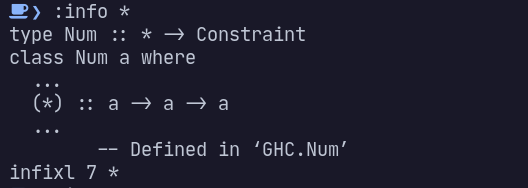
\includegraphics[width=8 cm]{img/2022-06-20-20-56-17.png}
 \end{center} 
 \begin{itemize} \renewcommand\labelitemi{\small \textcolor{Lavender}{$\blacksquare$}}
  \item Use {\fontfamily{cmtt}\selectfont space}, not Tab.
  \item All declarations in the module must start at the \textbf{same column}.
   The first declaration in a module defines the remaining ones.
 \item \textbf{Sectioning} {\fontfamily{cmtt}\selectfont (+1), (*30), ...}       
 \end{itemize}

   
   % (quot x y) * y + (rem x y) == x
   % (div x y) * y + (mod x y) == x
   %
   % mod has the same sign as the divisor.
   % rem: dividend
   %


   \section{Let and where}
   \begin{multicols}{2}
\begin{itemize} \renewcommand\labelitemi{\small \textcolor{Lavender}{$\blacksquare$}}
  \item 
   {\fontfamily{cmtt}\selectfont Let} introduces an expression 
 \item {\fontfamily{cmtt}\selectfont where} is a declaration.
\item \textbf{Scope.} The area of \textit{source code} where a binding of a variable applies. 
\item The \textbf{order} in code is unimportant.
\end{itemize}
   \end{multicols}      
   {\fontfamily{cmtt}\selectfont where}: syntactic sugar for a declaration.

       \textbf{Syntactic sugar} is syntax within a programming language designed to make expressions easier
       to write or read.
    







\end{document}
